\documentclass{article}

\usepackage{amsmath}
\usepackage{titling}
\usepackage{listings}
\usepackage{polski}
\usepackage{hyperref}
\usepackage{tablefootnote}
\usepackage{svg}
\usepackage[output-decimal-marker={,}]{siunitx}
\usepackage[a4paper, margin=2cm]{geometry}

\title{Technologie Sieciowe - Laboratorium}
\posttitle{\par\end{center}\begin{center}
    Lista nr 1 - Ping, Traceroute, WireShark 
\end{center}}
\date{21 marca 2022}
\author{Krzysztof Nowak (260055)}




\lstset{frame=single, breaklines}

\begin{document}
    \maketitle

    \section{Ping}
    Program Ping jest narzędziem diagnostycznym korzystającym z protokołu ICMP. Wysyła pakiety żądania echa do badanego hosta, który odsyła odpowiedzi. Służy przede wszystkim do sprawdzania czy istnieje połączenie do testowanego hosta oraz mierzenia występujących opóźnień i utraty pakietów.

Przykładowe wywołanie polecenia ping do serwera naszej katedry:
    \begin{lstlisting}
$ ping cs.pwr.edu.pl -c 2
PING cs.pwr.edu.pl (156.17.7.22) 56(84) bytes of data.
64 bytes from informatyka.im.pwr.wroc.pl (156.17.7.22): icmp_seq=1 ttl=58 time=3.97 ms
64 bytes from informatyka.im.pwr.wroc.pl (156.17.7.22): icmp_seq=2 ttl=58 time=3.59 ms

--- cs.pwr.edu.pl ping statistics ---
2 packets transmitted, 2 received, 0% packet loss, time 1001ms
rtt min/avg/max/mdev = 3.594/3.780/3.966/0.186 ms
    \end{lstlisting}

    \subsection{Badanie liczby węzłów na trasie}
    Datagramy IPv4 i IPv6 posiadają pole Time to live (TTL). Wartość ta jest ustawiana przez nadawcę pakietu, a następnie dekrementowana przez każdy węzeł, przez który przechodzi datagram. Gdy TTL osiągnie 0, pakiet jest usuwany. Możemy wykorzystać tą własność do określenie liczby węzłów na trasie, poprzez znalezienie minimalnej wartości TTL. Zmierzmy "odległość" do hosta cs.pwr.edu.pl
    
\begin{lstlisting}
$ ping cs.pwr.edu.pl -c 1 -t 7
PING cs.pwr.edu.pl (156.17.7.22) 56(84) bytes of data.
From 156.17.33.1 (156.17.33.1) icmp_seq=1 Time to live exceeded

--- cs.pwr.edu.pl ping statistics ---
1 packets transmitted, 0 received, +1 errors, 100% packet loss, time 0ms
\end{lstlisting}

    \begin{lstlisting}
$ ping cs.pwr.edu.pl -c 1 -t 8
PING cs.pwr.edu.pl (156.17.7.22) 56(84) bytes of data.
64 bytes from informatyka.im.pwr.wroc.pl (156.17.7.22): icmp_seq=1 ttl=58 time=3.73 ms

--- cs.pwr.edu.pl ping statistics ---
1 packets transmitted, 1 received, 0% packet loss, time 0ms
rtt min/avg/max/mdev = 3.734/3.734/3.734/0.000 ms
    \end{lstlisting}



    Widzimy, że otrzymujemy odpowiedź na ping z TTL=8, podczas gdy dla TTL=7 otrzymujemy informację od ostatniego węzła na trasie o wyzerowaniu licznika TTL i usunięciu pakietu. Zatem odległość do tego hosta wynosi 8 węzłów.

    Możemy również oszacować odległość w drugą stronę, od badanego hosta. Wartości TTL z jakimi wysyłane są pakiety odpowiedzi, zależą od systemu operacyjnego i konfiguracji badanego hosta. Typowe wartości to: 30, 32, 60, 64, 128, 200, 254, 255. \footnote{\url{http://subinsb.com/default-device-ttl-values/}}

    Odejmując wartość TTL odebranego pakietu od wartości, z którą spodziewamy się, że został nadany, otrzymujemy liczbę węzłów na trasie od hosta badanego. Dla powyższego pinga, odległość powrotna wynosi prawdopodobnie: $64 - 58 = 6$. 

    \subsection{Wyniki pomiarów}
    Powyższe pomiary przeprowadziłem dla kilku hostów. Czas został zmierzony dla $n=20$ zapytań. Pomiary wykonywałem z Wrocławia.
    

    \begin{table}[h!]
        \caption{Pomiar czasu i liczby przeskoków przy pomocy polecenia ping}
        \label{tab:ping1}
        \centering
        \begin{tabular}{|c|c|p{3cm}|p{3cm}|c|}
            \hline
            Adres hosta & Średni czas [ms] & Liczba przeskoków do hosta & Liczba przeskoków od hosta & Lokalizacja\\
            \hline
            cs.pwr.edu.pl & $\num{3,33} \pm \num{0,55}$ & 8 & 6 & Wrocław\\
            \hline 
            pg.edu.pl & $\num{9,7} \pm \num{2,0}$ & 13 & 12 & Gdańsk \\
            \hline
            ed.ac.uk & $\num{53,02} \pm \num{0,45}$ & 16 & 20 & Edynburg, Szkocja\\
            \hline
            13.225.209.13 \tablefootnote{Znalezione przez Jakuba Karwowskiego} & $\num{100,91} \pm \num{0,71}$ & 31 & 20 & USA\\
            \hline
            catalog.mit.edu & $141 \pm 13$ & 12 & 17 & Massachusetts, USA \\
            \hline
            zealvps.com & $\num{341.24} \pm \num{0,63}$& 17 & 17 & Nowa Zelandia\\
            \hline
            103.178.35.1 & $\num{302,70} \pm \num{0,76}$ & 35& 15 & Antarktyda \\
            \hline
        \end{tabular}
    \end{table}

    Najdalszy host (103.178.35.1) pod względem liczby węzłów, jaki udało mi się znaleźć, oddalony był o 35 skoków. Możemy przyjąć, że "średnica internetu" jest liczbą tego rzędu. 

    Najdalszy pod względem opóżnienia host jaki udało mi się znaleźć to zealvps.com - dostawca serwerów znajdujący się w Nowej Zelandi. Średnie opóżnienie wyniosło aż $341~ms$.

    Hosty 103.178.35.1 oraz 13.225.209.13 prawdopodobnie znajdują się w sieciach wirtualnych. Wskazuje na to wysoka asymetria, pomiędzy pakietami poruszającymi się w głąb sieci, względem pakietów opuszczających oraz w przypadku 13.225.209.13, liczba przeskoków jest o 10 większa niż dla catalog.mit.edu, który ma podobne opóźnienie i geolokalizację. Może to sugerować, że skoki to odbyły się jedynie wirtualnie.

    \subsection{Długość pakietu}
    Pakiet ICMP Ping składa się z nagłówka o długości 8 bajtów oraz $n$ bajtów danych. Połączenia między poszczególnymi hostami mają ustalone MTU, czyli maksymalną długość ramki, jaka może zostać przesłana. W wypadku, gdy ramka jest dłuższa niż MTU, pakiet zostanie zfragmentowany. Protokół IPv4 umożliwa zaznaczenie flagi wyłączającej możliwość fragmentowania. Wtedy ramki dłuższe od MTU zostaną odrzucone. Zbadajmy wpływ rozmiaru pakietów na czasy opóźnień. Na rys. \ref{fig:cspwr} przedstawiono wynik pomiarów dla domeny cs.pwr.edu.pl, znajdującej się w obrębie sieci miejskiej. Pakiety nie fragmentowane mają opóźnienia niemalże stałe. Opóźnienie zwiększa się wraz ze wzrotstm długości pakietu, osiągając wartość o $12~ms$ większą niż początkowa dla $n=65\cdot10^3$.

    Sytuacja wygląda podobnie dla pozostałych hostów.
    \begin{figure}[h!]
        \includesvg{cspwr.svg}
        \label{fig:cspwr}
        \caption{Wpływ rozmiaru ładunku na czas odpowiedzi dla hosta cs.pwr.edu.pl}
    \end{figure}

    \begin{figure}[h!]
        \includesvg{ZEAL.svg}
        \caption{Wpływ rozmiaru ładunku na czas odpowiedzi dla hosta zealvps.com}
    \end{figure}

    \begin{figure}[h!]
        \includesvg{edacuk.svg}
        \caption{Wpływ rozmiaru ładunku na czas odpowiedzi dla hosta ed.ac.uk}
    \end{figure}

    \newpage
 ~
    \newpage
\section{Traceroute}
Polecenie \texttt{traceroute} wykorzystuje TTL do badania trasy pakietów. Wysyłane są wiadomości o kolejnych, rosnących wartościach TTL zaczynając od 1. Powoduje to, że host, znajdujący się tyle przeskoków w głąb trasy, odsyła wiadomość błędu, wraz z własnym adresem. Pozwala to na ustalenie przez jakie węzły kolejno przechodzą pakiety zaadresowane do danego hosta. Poniżej przedstawiono badanie trasy do hosta cs.pwr.edu.pl znajdującego się w obrębie wrocławskiej sieci miejskiej. Widoczne są węzły należące do Netii (mojego dostawcy internetu) oraz Wrocławskiej Akademickiej Sieci Komputrowej.

\begin{lstlisting}
$ traceroute cs.pwr.edu.pl
traceroute to cs.pwr.edu.pl (156.17.7.22), 30 hops max, 60 byte packets
 1  _gateway (192.168.1.1)  1.104 ms  1.395 ms  1.507 ms
 2  83.238.252.80 (83.238.252.80)  4.192 ms  4.168 ms  4.164 ms
 3  wrocc002rt09.inetia.pl (83.238.113.28)  10.588 ms  6.697 ms  4.070 ms
 4  POZNH002RT09.inetia.pl (83.238.249.150)  4.780 ms  4.957 ms  4.949 ms
 5  centrum-rtr-sniezka.wask.wroc.pl (156.17.251.167)  11.887 ms  12.143 ms  5.163 ms
 6  z-wask2-do-pwr2.pwrnet.pwr.wroc.pl (156.17.18.244)  6.115 ms  5.216 ms  5.134 ms
 7  156.17.33.1 (156.17.33.1)  5.240 ms  4.418 ms  4.375 ms
 8  informatyka.im.pwr.wroc.pl (156.17.7.22)  3.916 ms  4.176 ms  4.217 ms
\end{lstlisting}

Często zdarza się, że niektóre węzły nie wysyłają wiadomości, podczas wyzerowania TTL. Dzieje się tak na przykładzie poniżej. Umożliwia to ustalenie trasy do badanego hosta.
\begin{lstlisting}
$ traceroute 103.178.35.1
traceroute to 103.178.35.1 (103.178.35.1), 30 hops max, 60 byte packets
 1  _gateway (192.168.1.1)  1.120 ms  1.075 ms  1.175 ms
 2  83.238.252.80 (83.238.252.80)  4.058 ms  4.437 ms  4.611 ms
 3  wrocc002rt09.inetia.pl (83.238.113.28)  6.934 ms  6.245 ms  6.449 ms
 4  sp75-cp.pie.warszawa.sint.pl (213.195.141.51)  9.782 ms  9.977 ms  9.953 ms
 5  ae3-2072.lon10.core-backbone.com (80.255.15.166)  27.050 ms  27.315 ms  27.267 ms
 6  core-backbone.cdn77.com (5.56.17.178)  32.822 ms  31.063 ms  31.048 ms
 7  v3518.cr02.lon07.gb.misaka.io (156.146.32.107)  32.113 ms  31.265 ms  32.464 ms
 8  po-04.lag.lon07.gb.misaka.io (45.142.244.4)  31.592 ms  31.287 ms  31.567 ms
 9  * * *
10  * * *
11  * * *
12  * * *
13  * * *
14  * * *
\end{lstlisting}

Poniżej przedstawiono przykład połączenia do MIT w Ameryce. Szczególnie ciekawy jest odcinek między węzłami 4 a 6, ponieważ jest to połączenie między Katowicami a Chicago.
\begin{lstlisting}
$ traceroute catalog.mit.edu
traceroute to catalog.mit.edu (12.2.169.180), 30 hops max, 60 byte packets
 1  _gateway (192.168.1.1)  0.990 ms  1.005 ms  1.485 ms
 2  83.238.252.80 (83.238.252.80)  3.745 ms  3.785 ms  3.754 ms
 3  wrocc002rt09.inetia.pl (83.238.113.28)  11.009 ms  10.705 ms  10.872 ms
 4  JAWOH001RT09.inetia.pl (83.238.249.43)  12.278 ms  12.399 ms  12.362 ms
 5  * * *
 6  ae0.11.edge1.Chicago10.level3.net (4.69.219.17)  135.755 ms ae2.2.edge1.Chicago10.level3.net (4.69.133.29)  135.435 ms  135.334 ms
 7  ATT-level3-Chicago2.Level3.net (4.68.37.86)  137.541 ms  140.494 ms  140.140 ms
 8  cr2.cgcil.ip.att.net (12.122.132.198)  140.159 ms  140.907 ms  138.812 ms
 9  okbil81crs.ip.att.net (12.122.1.193)  137.144 ms  142.018 ms  142.768 ms
10  12.122.151.245 (12.122.151.245)  136.091 ms  135.420 ms  134.798 ms
11  12.247.128.154 (12.247.128.154)  141.956 ms  141.057 ms  142.569 ms
12  clpublic2-host80.leepfrog.com (12.2.169.180)  142.293 ms !X  142.481 ms !X  140.943 ms !X

\end{lstlisting}
    \section{WireShark}
    WireShark jest narzędziem służącym do przechwytywania i analizy pakietów sieciowych (a także innych, jak USB lub DBUS).
    Można wykorzystać go do debugowania własnych aplikacji sieciowych, diagnozowania ruchu sieciowego lub inżynierii odwrotnej protokołów.
    Przechwytywane pakiety mogą nie tylko być związane z komputerem, na którym uruchomiony jest program, lecz możliwe jest analizowanie danych przechwytywanych np. na routerze przy użyciu  \texttt{tcpdump} lub przechodzących przez odpowiednio zmostkowane połączenie.
    Na rys. \ref{fig:shark} przedstawiono zrzut z ekranu programu, wykorzystanego do przechwycenia logowania przy użyciu nieszyfrowanego połączenia HTTP. W wiadomości POST możemy znaleźć login i hasło przesłane jawnym tekstem.
    \begin{figure}[h!]
        \centering
        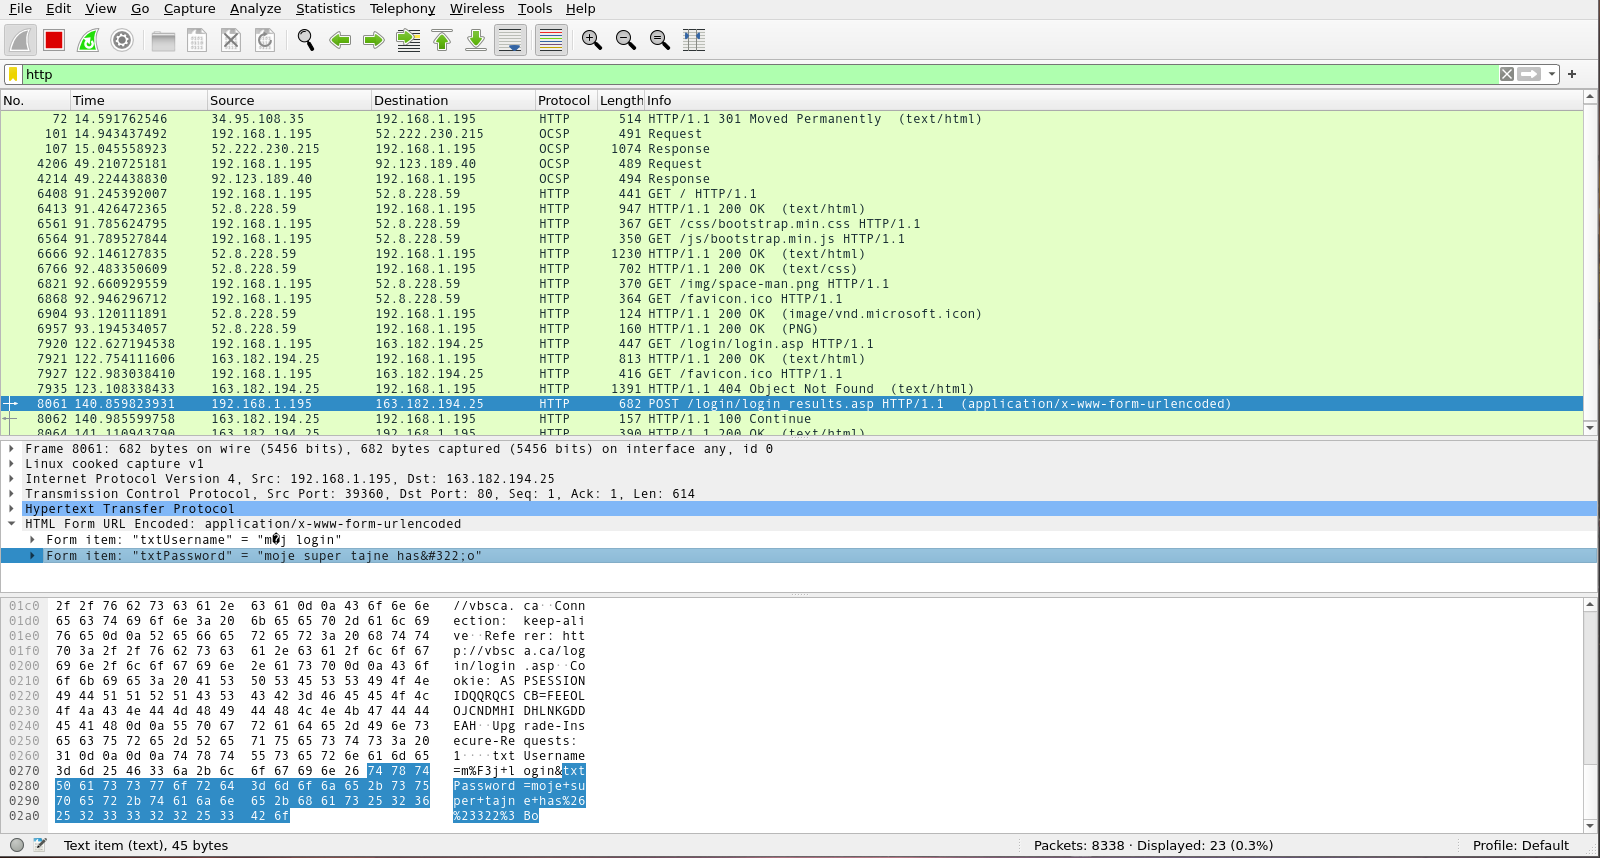
\includegraphics[width=17cm]{wireshark.png}
        \caption{Przykład użycia WireSharka do przechwycenia HTTP POST}
        \label{fig:shark}
    \end{figure}
\end{document}